\documentclass[12pt,a4paper]{article}
\usepackage[utf8]{inputenc}
\usepackage[T2A]{fontenc}
\usepackage[ukrainian]{babel}
\usepackage{fancyvrb}
\usepackage{pdflscape}

\usepackage{amsmath} % у преамбулі
\usepackage{array, multirow}
\usepackage{hyperref} % <-- Обов'язково підключіть цей пакет
\usepackage{caption}
\usepackage{booktabs}
\usepackage{subcaption} % для підписів (а), (б)
\usepackage{breqn} % Пакет для автоматичного перенесення виразів
\usepackage{mathtools} % Для додаткових можливостей, наприклад, для створення кастомних конструкцій
\usepackage{makecell} % Для створення багаторядкових комірок у таблицях
\usepackage{enumitem}

\usepackage{xcolor}

\renewcommand{\thetable}{№\arabic{table}}
\captionsetup[table]{name=Таблиця}  % замість "Табл." буде "Таблиця"

\usepackage{graphicx} % <-- Для роботи з \includegraphics
\usepackage{geometry}
\geometry{
    left=2cm,
    right=2cm,
    top=2cm,
    bottom=2cm
}


\begin{document}

    \begin{titlepage}

        \thispagestyle{empty}
        \begin{center}
        \large
        Національний технічний університет України\\
        «Київський політехнічний інститут імені Ігоря Сікорського»\\[1em]
        Факультет інформатики та обчислювальної техніки\\
        Кафедра загальної фізики
        \end{center}

        \vfill

        \begin{center}
        \textbf{\LARGE Фізика}\\[2em]
        \textbf{\Large Лабораторна робота №3-5}\\
        «Вивчення поляризованого світла» 
        \end{center}

        \vfill

        \begin{flushright}
        Виконав: студент 1 курсу ФІОТ, гр. ІО-41\\
        \textit{Давидчук А. М.}\\
        Залікова книжка № 4106\\[1em]
        Перевірив: \textit{Колган В.\,В.}
        \end{flushright}

        \vfill

        \begin{center}
        Київ -- 2025
        \end{center}

    \end{titlepage}

    \setlength{\parindent}{0pt}

    \textbf{\underline{Тема:}} «Вивчення поляризованого світла».

    \vspace{1em}

    \textbf{\underline{Мета:}} експериментальне перевірити формули Френеля, досліджуючи
    відбивання поляризованого світла від скляної пластинки, та визначити кут
    Брюстера, показник заломлення скла та площину коливань світлового вектора $\vec{E}$.

    \vspace{1.5em}

    \begin{center} \textbf{\large Теоретичні відомості} \end{center}
    \setlength{\parindent}{1.5em}

    \begin{center} \textbf{Природне і поляризоване світло. Поляризатори} \end{center}

    Як відомо, світло являє собою поперечну електромагнітну хвилю. Світлові хвилі
    бувають природними та поляризованими, тобто такими, в яких (на відміну від
    природних) коливання вектора $\vec{E}$ певним чином упорядковані. Способи
    впорядкування, а у відповідності до них і види поляризації. Оптичні пристрої, за
    допомогою яких світло поляризується, називаються поляризаторами.

    \begin{center} \textbf{Відбивання плоскої лінійно поляризованої хвилі від діелектричної пластинки.} \end{center}

    При розгляді цього питання хвилю, що падає, представляють у вигляді
    суперпозиції двох хвиль \(\vec{E}_{\parallel 0}\) та \(\vec{E}_{\perp 0}\), електричні вектори яких коливаються відповідно у
    площині падіння хвилі та перпендикулярно до неї (див. рис. 5.1).

    \begin{figure}[!ht]

        \renewcommand{\thefigure}{5.\arabic{figure}} % робимо "3.1", "3.2" і т.д.

        \centering
        % Підставляєте потрібний шлях та розмір зображення:
        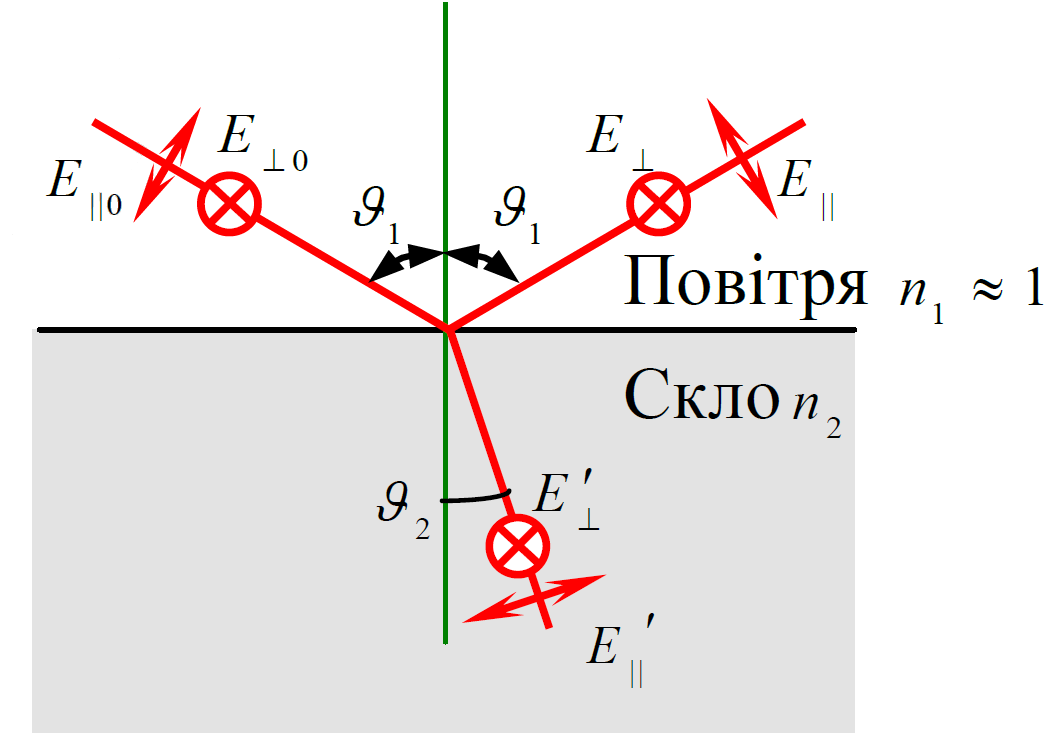
\includegraphics[width=0.4\textwidth]{5.1.png}
        % Підпис (зазвичай під малюнком):
        \caption{}
        % Мітка для посилань у тексті (\ref{fig:...})
        \label{fig1:schema}

    \end{figure}

    Залежність амплітуди
    відбитої й заломленої хвиль від кута падіння описується формулами Френеля.

    Тут $n_1, n_2$ --- абсолютні показники заломлення повітря й скла;
    $\vartheta_1, \vartheta_2$ --- кути падіння і заломлення хвилі.

    Так, наприклад, амплітуди відбитих хвиль \(\vec{E}_{\parallel 0}\) та \(\vec{E}_{\perp 0}\) відповідно до цих формул

    \begin{equation}
        E_{\parallel}
        =E_{\parallel0}\,\frac{\tg(\vartheta_1-\vartheta_2)}{\tg(\vartheta_1+\vartheta_2)},
        \quad
        E_{\perp}
        =E_{\perp0}\,\frac{\sin(\vartheta_1-\vartheta_2)}{\sin(\vartheta_1+\vartheta_2)}.
        \tag{5.1}
    \end{equation}

    по різному залежать від кута падіння $\vartheta_1$.

    З формул Френеля (5.1) видно, що за умови $\vartheta_1 = \vartheta_2 = \pi \slash 2$
    амплітуда, відбитої хвилі $E_{\parallel}$ стає рівною нулю, і відбите світло містить лише компонент
    $E_{\perp}$, тобто воно є повністю
    поляризованим. Величина кута падіння, при якому це відбувається, визначається з
    умови $\tg \vartheta_{\text{Бр}} = n_2 / n_1$. Ця умова носить назву умови Брюстера, або ж закону Брюстера.

    Оскільки кути $\vartheta_1, \vartheta_2$, які фігурують у (5.1), пов'язані законом заломлення світла
    $\left( \sin \vartheta_1 \right.$ $\left. \slash \sin \vartheta_2 = n_2 / n_1 \right)$
    кут $\vartheta_2$ можна виразити через $\vartheta_1$ і, таким чином, одержати функцію,
    яка описує залежність амплітуди відбитих хвиль від кута падіння
    $\vartheta_1$.

    \newpage

    На рис. 5.2 показані графіки функції $E_{\parallel} / E_0 = f(\vartheta_1)$ (крива I)
    та $E_{\perp} / E_0 = f(\vartheta_1)$ (крива II),
    розраховані для випадку, коли $n_1 = 1, n_2 = 1{,}5$.

    \begin{figure}[!ht]

        \renewcommand{\thefigure}{5.\arabic{figure}} % робимо "3.1", "3.2" і т.д.

        \centering
        % Підставляєте потрібний шлях та розмір зображення:
        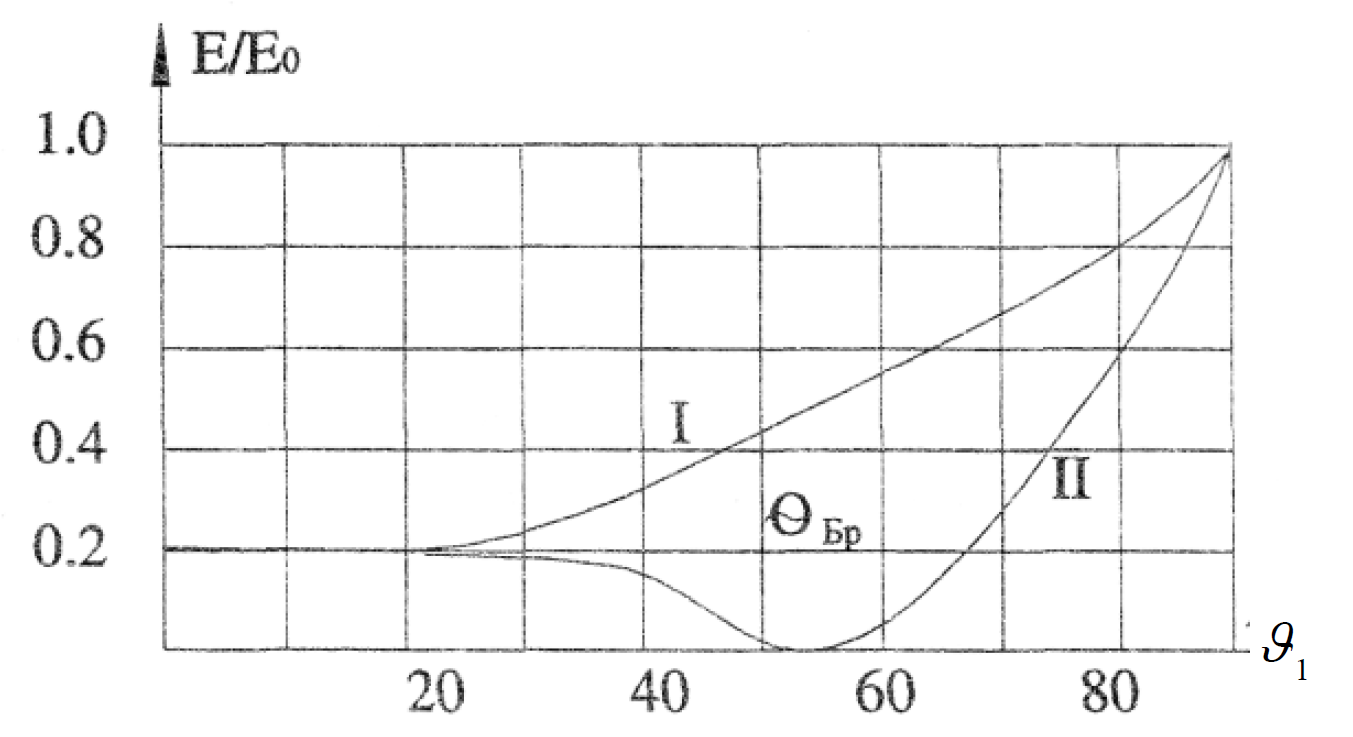
\includegraphics[width=0.4\textwidth]{5.2.png}
        % Підпис (зазвичай під малюнком):
        \caption{}
        % Мітка для посилань у тексті (\ref{fig:...})
        \label{fig2:schema}

    \end{figure}

    Як з рис. 5.2, криві залежностей для $\perp$ та $\parallel$ поляризацій вектора напруженості $\vec{E}$
    суттєво різняться, що дозволяє за результатами експерименту встановити площину
    поляризації хвилі, яка падає на скло, величину кута Брюстера та показник заломлення
    скла.

    \begin{center} \textbf{Проходження лінійно поляризованої хвилі через поляризатор. Закон Малюса} \end{center}

    Якщо лінійно поляризована світлова хвиля падає нормально на поляризатор так,
    що площина коливань її вектора $\vec{E}$ складає з головною оптичною площиною
    поляризатора (11) кут $\alpha$, то інтенсивність $I$ хвилі, що пройшла, визначається
    виразом

    \begin{equation}
        I = I_0 \cos^2 \alpha,
        \tag{5.2}
    \end{equation}

    де $I_0$ --- інтенсивність світла, що падає. Це співвідношення називається законом Малюса.
    Знаючи площину поляризатора та оцінюючи інтенсивність світла, що пройшло, можна
    за законом Малюса встановити площину коливань досліджуваного лінійно
    поляризованого світла.

    \begin{center} \textbf{\large Практична частина} \end{center}

    \begin{center} \textbf{Методика вимірювання інтенсивності та амплітуди світлової хвилі} \end{center}

    Під інтенсивністю світла розуміють усереднену величину модуля
    густини потоку енергії світлової хвилі

    \begin{equation}
        I = \left\langle \left| \vec{S} \right| \right\rangle = \frac{1}{2} \sqrt{\frac{\varepsilon_0}{\mu_0}}E_m^2,
        \tag{5.3}
    \end{equation}

    де $\varepsilon_0, \mu_0$ --- відповідно електрична і магнітна сталі,
    $E_m$ --- амплітуда світлової хвилі.

    Інтенсивність і амплітуда світлової хвилі у цій роботі вимірюються за допомогою
    приймача випромінювання, в якому використовується вентильний фотоефект.

    Приймач складається з фотоелектричного датчика, що перетворює світловий
    потік у фотоЕРС, і вольтметра для вимірювання останньої.

    Пропорційність між фотоЕРС та інтенсивністю світлової хвилі (за малих
    інтенсивностей) забезпечується законами внутрішнього фотоефекту.

    Таким чином, інтенсивність світлової хвилі виявляється пропорційною показам
    вольтметра $I \sim U$, а її амплітуда --- кореню квадратному з показань приладу
    $E_m \sim \sqrt{U}$.

    \textbf{Визначення виду поляризації світлової хвилі}

    Для прикладу розглянемо методику ідентифікації лише лінійно поляризованої хвилі.

    Лінійно поляризована хвиля легко пізнається, якщо пропускати її крізь
    поляризатор. Як відмічалося раніше, інтенсивність хвилі, що пройшла, у цьому випадку
    підпорядкована закону Малюса: $I = I_0 \cos^2 \alpha$.

    Обертаючи аналізатор у площині,
    нормальній до напрямку поширення хвилі, можна знайти два його характерні
    положення: у першому інтенсивність світла , що пройшла, максимальна, у другому
    (відрізняється на $90^{\circ}$ від першого) --- нульова. Для більшої переконливості закон (5.2)
    може бути перевіреним у повному об'ємі.

    \begin{center} \textbf{Опис експериментальної установки} \end{center}

    Основною деталлю експериментальної
    установки є вимірювальна головка з оптичними
    елементами та лімбом 1 (рис. 5.3).

    \begin{figure}[!ht]

        \renewcommand{\thefigure}{5.\arabic{figure}} % робимо "3.1", "3.2" і т.д.

        \centering
        % Підставляєте потрібний шлях та розмір зображення:
        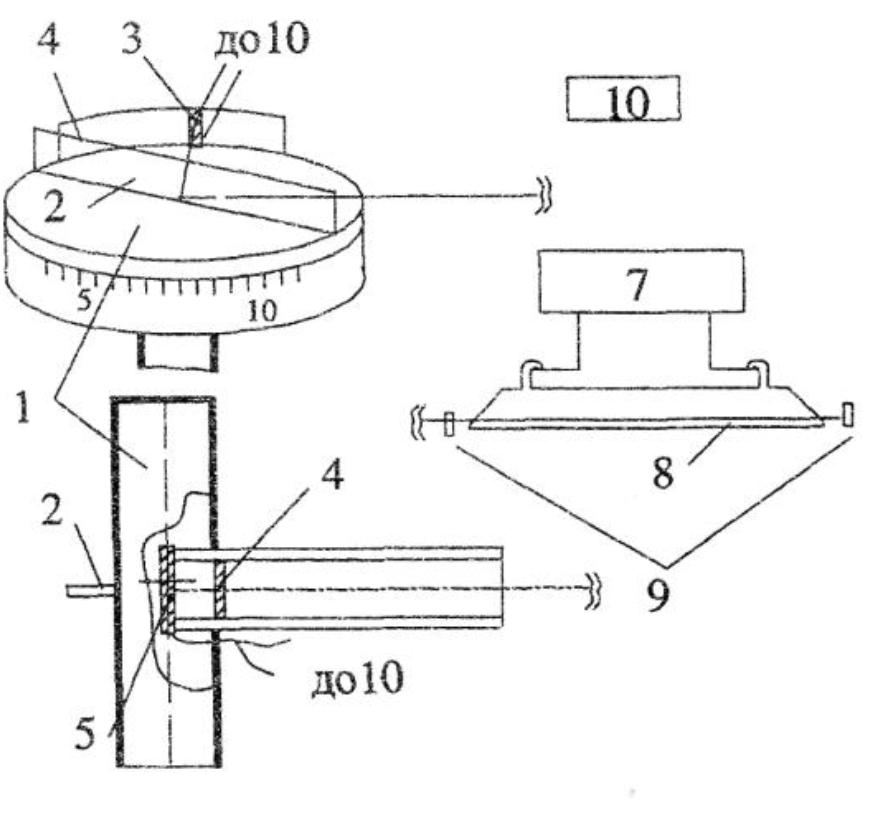
\includegraphics[width=0.4\textwidth]{5.3.png}
        % Підпис (зазвичай під малюнком):
        \caption{}
        % Мітка для посилань у тексті (\ref{fig:...})
        \label{fig3:schema}

    \end{figure}

    Головка може бути встановлена у двох положеннях:

    \begin{enumerate}[label=\alph*)]
        \item вертикально для зняття залежності амплітуди відбитої хвилі від кута падіння;
        \item горизонтально для перевірки закону Малюса і виду поляризації світлової хвилі.
    \end{enumerate}

    У верхній частині головки встановлені
    плоскопаралельна пластинка 2, фотоприймач 3,
    екран 4. У нижній її частині --- поляроїд 6 та
    другий фотоприймач 5. Фотоприймачі з'єднані з
    вольтметром 10.

    Джерелом поляризованого світла є He-Ne
    лазер. У ньому є джерело живлення 7, газорозрядна трубка 8 яка знаходиться між
    дзеркалами резонатора 9.

    Довжина хвилі лазерного випромінювання $\lambda = 0{,}63$ мкм,
    розходження пучка $30^{\circ}$ потужність $\sim 1$ МВт.

    На передньому торці лазера намальовані взаємно перпендикулярні лінії І і II.
    Уздовж однієї з них відбувається коливання світлового вектора $\vec{E}$ . В установці
    передбачена можливість зміни напрямку коливань світлового вектора відносно
    діелектричної пластинки (скло) шляхом обертання лазера навколо своєї осі.

    Увага! Попадання в очі прямого лазерного пучка небезпечно для зору! Світло лазера
    можна спостерігати тільки після відбиття від поверхонь, що розсіюють.

    \newpage

    \begin{center} \textbf{Порядок виконання} \end{center}

    \begin{enumerate}
        \item Ознайомився з експериментальною установкою: He-Ne лазер, поляризатори, фотоприймачі, вольтметр.
        \item У вертикальному положенні установки зняв залежності амплітуд $E_{\perp}/E_{\perp0}$ та $E_{\parallel}/E_{\parallel0}$ від кута падіння світла.
        \item Зафіксував напругу для кожного кута, обчислив амплітуду за формулою $E \propto \sqrt{U}$.
        \item Побудував графіки експериментальної та теоретичної залежностей для $E_{\perp}$ і $E_{\parallel}$.
        \item Для розрахунку теоретичних амплітуд скористався формулами Френеля:
        \[
          \frac{E_{\parallel}}{E_{\parallel 0}} = \frac{\tg(\theta_1 - \theta_2)}{\tg(\theta_1 + \theta_2)}, \quad
          \frac{E_{\perp}}{E_{\perp 0}} = \frac{\sin(\theta_1 - \theta_2)}{\sin(\theta_1 + \theta_2)}
        \]
        де $\theta_2 = \arcsin\left(\frac{n_1}{n_2} \sin \theta_1\right)$ згідно із законом заломлення.
        \item Визначив кут Брюстера з графіка та обчислив показник заломлення скла за формулою:
        \[
          n = \tg \vartheta_{\text{Бр}}
        \]
        \item Перевів установку у горизонтальне положення.
        \item Провів вимірювання залежності інтенсивності світла, що проходить через аналізатор, від кута повороту поляризатора.
        \item Побудував графік $U$ від $\cos^2 \alpha$ та перевірив виконання закону Малюса:
        \[
          I = I_0 \cos^2 \alpha, \quad I \propto U
        \]
        \item Узагальнив результати, зробив висновки щодо підтвердження формул Френеля, закону Брюстера і закону Малюса.
      \end{enumerate}

    \newpage

    \begin{landscape}

    Під час обчислення експериментальних значень відношень амплітуд, користуватимемось тим, що $E \propto \sqrt{I} \propto \sqrt{U}$.
    Тобто щоб знайти відношення 2 амплітуд (довільної та максимальної), ми повинні знайти відношення квадратів напруг (при довільній та максимальній амплітуді).

    Під час обчислення теоретичних значень відношень амплітуд за формулою 5.1, ми приймаємо $n_1 = 1, n_2 = 1{,}5$, звідси кут відбиття $\vartheta_2$ замінимо на
    \[
    \vartheta_2 = \arcsin \left(\frac{n_1}{n_2} \sin \vartheta_1\right) = \arcsin \left(\frac{2}{3} \sin \vartheta_1\right)
    \]

    звідси

    \[
    E_{\parallel}
    =E_{\parallel0}\,\frac{\tg\left(\vartheta_1-\arcsin \left(\dfrac{2}{3} \sin \vartheta_1\right)\right)}{\tg\left(\vartheta_1+\arcsin \left(\dfrac{2}{3} \sin \vartheta_1\right)\right)},
    \quad
    E_{\perp}
    =E_{\perp0}\,\frac{\sin\left(\vartheta_1-\arcsin \left(\dfrac{2}{3} \sin \vartheta_1\right)\right)}{\sin\left(\vartheta_1+\arcsin \left(\dfrac{2}{3} \sin \vartheta_1\right)\right)}.
    \]

    \begin{table}[ht]
        \centering
        \begin{tabular}{|l|l|l|l|l|l|l|l|l|l|}
        \hline
        \multirow{2}{*}{Орієнтація вектора} & \multicolumn{9}{l|}{Кут}                     \\ \cline{2-10}
                                            & $\vartheta^{\circ}$ & 10 & 20 & 30 & 40 & 50 & 60 & 70 & 80 \\ \hline
        \multirow{3}{*}{$\perp, U_{\perp0} = 276{,}85$ В}               & $U$     & 25,28 &  28,43  &  32,88  &  41,44  &  55,16  &  78,00  &  155,61  &  176,97  \\ \cline{2-10}
                                            & $\sqrt{U}$ &  5,0279  &  5,3320  &  5,7341  &  6,4374  &  7,4270  &  8,8318  &  12,4744  &  13,3030  \\ \cline{2-10}
                                            & $E_{\perp} / E_{\perp0}$   &  0,3022  &  0,3205  &  0,3446  &  0,3869  &  0,4464  & 0,5308  & 0,7497 & 0,7995  \\ \hline
        Теоретичне
        значення                     & $E_{\perp} / E_{\perp0}$   &  0,2041  &  0,2170  &  0,2404  &  0,2778  & 0,3347   &  0,4202  &  0,5474  &  0,7339  \\ \hline
        \multirow{3}{*}{$\parallel, U_{\parallel0} = 238{,}72$ В}        & $U$    &  20,42  &  18,28  &  14,77  &  9,85  &  4,17  &  0,12  &  5,63  & 48,39   \\ \cline{2-10}
                                            & $\sqrt{U}$ &  4,5188  &  4,2755  & 3,8432  &  3,1385  &  2,0421  & 0,3464   &  2,3728  & 6,9563   \\ \cline{2-10}
                                            & $E_{\parallel} / E_{\parallel0}$ & 0,2925   &   0,2767  &   0,2487 &  0,2031  &  0,1322  &  0,0224  &  0,1536  &  0,4502  \\ \hline
        Теоретичне
        значення                     & $E_{\parallel} / E_{\parallel0}$  &  0,1959  &  0,1829  &  0,1589  &  0,1196  &  0,0572  &  -0,0424  &  -0,2061  & -0,4866  \\ \hline
        \end{tabular}
        \caption{Таблиця завдання №1}
    \end{table}

    Всі обчислення проводились за допомогою Python коду (Лістинг 1.1)

    $U_{max}$ --- значення напруги $U$ при 0 градусів, і дорівнює $U_{max} = 372{,}63$ В. І так як інтенсивність прямо пропорційна до напруги, то щоб знайти
    $\cos^2 \alpha$, я буду ділити кожне значення напруги при переміщенні кута на $U_{max}$ --- таким чином отримувати вектор експериментально виміряних величин.

    \end{landscape}

    \newpage

    TABLE 2

    \newpage

    Через те, що $n_1$ --- це показник заломлення повітря, і воно приблизно дорінює 1, то можемо сказати, що:

    \[
    \tg \vartheta_{\text{Бр}} \approx n_2 \Rightarrow \tg(57^{\circ}) \approx 1{,}54
    \]

    Що є дуже близьким до прийнятого в цій лабораторній $n_2 = 1{,}5$.

    Щодо виконання закону Малюса. Закон малюса:

    \[
    I = I_0 \cos^2 \alpha
    \]

    Звідси ми знаємо, що $I \propto U$, це значить, що $U \propto I_0 \cos^2 \alpha$, де $U$ --- функція, $\cos^2 \alpha$ --- аргумент, а $I_0$ --- коефіцієнт, тобто
    графік має вийти лінійним:

    \begin{figure}[ht]
        \centering
        \includegraphics[width=1.0\textwidth]{graph2.png}
    \end{figure}

    Експериментальні точки підпорядковуються лінійному рівнянню, тобто закон Малюса виконується, причому $I_0 \approx 372{,}62$ кандели.

    \vspace{1em}
    \setlength{\parindent}{0pt}

    \textbf{\underline{Висновок:}}

    \vspace{1em}

    У ході лабораторної роботи:
    
    \begin{itemize}
      \item Експериментально підтверджено формули Френеля для амплітуд відбитих компонент $E_{\parallel}$ та $E_{\perp}$.
      \item Визначено кут Брюстера: $\displaystyle \tg \vartheta_{\text{Бр}} = \frac{n_2}{n_1} \Rightarrow \vartheta_{\text{Бр}} \approx 57^\circ$, що відповідає $n_2 \approx 1{,}5$.
      \item Перевірено виконання закону Малюса: $I = I_0 \cos^2 \alpha$, графік $U \propto I_0\cos^2 \alpha$ є лінійним.
      \item Максимальна інтенсивність становить $I_0 \approx 372{,}62$ умов. од.
    \end{itemize}
    
    Отримані результати узгоджуються з теорією та підтверджують поляризаційні властивості світла.

    \newpage

    \begin{center}
        \textbf{\large Контрольні запитання}
    \end{center}

    \textit{1. Як можна уявити світлову хвилю? Основні характеристики монохроматичної хвилі.} \\ 

    Світлова хвиля — це поперечна електромагнітна хвиля, в якій електричний вектор $\vec{E}$ та магнітний вектор $\vec{B}$ коливаються перпендикулярно до напрямку поширення. Основні характеристики монохроматичної хвилі: довжина хвилі $\lambda$, частота $\nu$, амплітуда $E_m$, поляризація, фаза.

    \vspace{1em}

    \textit{2. Яке світло називається природним, а яке поляризованим? Чи може бути поляризованою повздовжня хвиля?} \\ 

    Природне світло — це неполяризоване світло, у якому напрямки коливань $\vec{E}$ змінюються хаотично. Поляризоване — світло з упорядкованим напрямком вектора $\vec{E}$. Повздовжня хвиля не може бути поляризованою, оскільки поляризація — це властивість лише поперечних хвиль.

    \vspace{1em}

    \textit{3. Які види поляризації світла ви знаєте? Що таке площина коливань?} \\ 

    Види поляризації: лінійна, кругова, еліптична. Площина коливань — це площина, в якій коливається вектор $\vec{E}$.

    \vspace{1em}

    \textit{4. Які ви знаєте поляризаційні пристрої? Що таке площина поляризатора?} \\ 

    Поляризаційні пристрої: поляроїди, дзеркала під кутом Брюстера, кристали (наприклад, турмалін). Площина поляризатора — площина, паралельна до напрямку коливань $\vec{E}$ після проходження через поляризатор.

    \vspace{1em}

    \textit{5. Що таке явище дихроїзму? Як воно використовується у поляризаторах?} \\ 

    Дихроїзм — це здатність деяких кристалів по-різному поглинати світло в залежності від напрямку поляризації. Використовується у поляроїдах для відсікання однієї з компонент $\vec{E}$.

    \vspace{1em}

    \textit{6. Яке світло називають частково-поляризованим?} \\ 

    Частково-поляризоване світло містить як впорядковану (поляризовану), так і випадкову (неполяризовану) компоненти.

    \vspace{1em}

    \textit{7. Що таке ступінь поляризації світла? Який смисл мають $I_{max}$ та $I_{min}$ ?} \\ 
    \[
    P = \frac{I_{\text{max}} - I_{\text{min}}}{I_{\text{max}} + I_{\text{min}}}
    \]
    $I_{\text{max}}$ — інтенсивність при максимальному пропусканні, $I_{\text{min}}$ — при мінімальному.

    \vspace{1em}

    \textit{8. Які є особливості проходження поляризованого світла крізь поляризатор? У чому полягає закон Малюса і як його можна одержати?} \\ 

    Інтенсивність змінюється за законом Малюса:
    \[
    I = I_0 \cos^2 \alpha
    \]
    де $\alpha$ — кут між площиною коливань світла та площиною поляризатора.

    \vspace{1em}

    \textit{9. Що таке $E_{\parallel}$ і $E_{\perp}$?} \\ 

    $E_{\parallel}$ — складова вектора $\vec{E}$ в площині падіння; $E_{\perp}$ — перпендикулярна до неї.

    \vspace{1em}

    \textit{10. Як виводяться формули Френеля?} \\ 

    Виводяться з умов неперервності $\vec{E}$ і $\vec{H}$ на межі поділу середовищ, використовуючи граничні умови Максвелла.

    \vspace{1em}

    \textit{11. Формули Френеля для відбитих і заломлених хвиль.} \\ 

    Для відбиття:
    \[
    \frac{E_{\parallel}}{E_{\parallel 0}} = \frac{\tg(\theta_1 - \theta_2)}{\tg(\theta_1 + \theta_2)}, \quad \frac{E_{\perp}}{E_{\perp 0}} = \frac{\sin(\theta_1 - \theta_2)}{\sin(\theta_1 + \theta_2)}
    \]
    Для заломлення — аналогічні співвідношення.

    \vspace{1em}

    \textit{12. Закон Брюстера. Його пояснення з точки зору електронної теорії.} \\ 

    При куті $\theta_{\text{Бр}}$, для якого $\tg \theta_{\text{Бр}} = \frac{n_2}{n_1}$, $E_{\parallel}$ не відбивається. Електронна теорія: відбите й заломлене $\vec{E}$ взаємно перпендикулярні — коливання електронів не збуджують відбиту хвилю.

    \vspace{1em}

    \textit{13. Фазові співвідношення між хвилею, що падає, відбитою та заломленою хвилями.} \\ 

    При відбитті можливий фазовий зсув на $\pi$ або його відсутність — залежно від поляризації та показників заломлення.

    \vspace{1em}

    \textit{14. Що таке звичайна та незвичайна хвиля? Покажіть площини їх коливань.} \\ 

    Звичайна хвиля — $\vec{E}$ перпендикулярний до оптичної осі; незвичайна — $\vec{E}$ лежить у площині, що містить оптичну вісь і напрям поширення.

    \vspace{1em}

    \textit{15. Сформулюйте принцип роботи оптичного квантового генератора.} \\ 

    Принцип вимушеного випромінювання: збуджений атом під дією фотона випромінює ще один — тієї ж фази, частоти й напрямку.

    \vspace{1em}

    \textit{16. Поясніть будову та принцип дії He-Ne лазера.} \\ 

    Газорозрядна трубка з He-Ne між дзеркалами резонатора. Збуджені атоми He передають енергію атомам Ne, які випромінюють світло. Світло багаторазово підсилюється між дзеркалами, формується когерентний пучок.

    \newpage

      \textbf{\large Код програми:}

      \vspace{1em}
  
      \small{ 

  \begin{verbatim}
import numpy as np
import math
from tabulate import tabulate

# Вектор кутів падіння у радіанах (переведення з градусів у радіани)
teta_vector = np.deg2rad(np.array([10, 20, 30, 40, 50, 60, 70, 80]))

# Початкове значення напруги для перпендикулярної компоненти
U0_perp = 276.85
# Вектор експериментальних значень напруги для перпендикулярної компоненти
U_perp_vector = np.array([25.28, 28.43, 32.88, 41.44, 55.16, 78.00, 155.61, 176.97])

# Початкове значення напруги для паралельної компоненти
U0_paral = 238.72
# Вектор експериментальних значень напруги для паралельної компоненти
U_paral_vector = np.array([20.42, 18.28, 14.77, 9.85, 4.17, 0.12, 5.63, 48.39])

# Обчислення для перпендикулярної компоненти
# Квадратний корінь з експериментальних значень напруги
sqrt_U_perp_vector = np.round(np.sqrt(U_perp_vector), 4)
# Експериментальне відношення амплітуд E_perp/E0
Eperp_E0_expr = np.round(sqrt_U_perp_vector / math.sqrt(U0_perp), 4)

# Теоретичне відношення амплітуд E_perp/E0 за формулами Френеля
k = 2/3  # Відношення показників заломлення n1/n2
Eperp_E0_theor = np.round(
    np.sin(teta_vector - np.arcsin(k * np.sin(teta_vector))) /
    np.sin(teta_vector + np.arcsin(k * np.sin(teta_vector))), 4
)

# Обчислення для паралельної компоненти
# Квадратний корінь з експериментальних значень напруги
sqrt_U_paral_vector = np.round(np.sqrt(U_paral_vector), 4)
# Експериментальне відношення амплітуд E_paral/E0
Eparal_E0_expr = np.round(sqrt_U_paral_vector / math.sqrt(U0_paral), 4)

# Теоретичне відношення амплітуд E_paral/E0 за формулами Френеля
Eparal_E0_theor = np.round(
    np.tg(teta_vector - np.arcsin(k * np.sin(teta_vector))) /
    np.tg(teta_vector + np.arcsin(k * np.sin(teta_vector))), 4
)

# Формування горизонтальної таблиці для виводу результатів
table_data = [
    ["U_perp"] + list(U_perp_vector),  # Експериментальні значення U_perp
    ["sqrt(U_perp)"] + list(sqrt_U_perp_vector),  # Квадратний корінь з U_perp
    ["E_perp/E0 EXPERIMENTAL"] + list(Eperp_E0_expr),  # Експериментальне E_perp/E0
    ["E_perp/E0 THEORETICAL"] + list(Eperp_E0_theor),  # Теоретичне E_perp/E0
    ["U_paral"] + list(U_paral_vector),  # Експериментальні значення U_paral
    ["sqrt(U_paral)"] + list(sqrt_U_paral_vector),  # Квадратний корінь з U_paral
    ["E_paral/E0 EXPERIMENTAL"] + list(Eparal_E0_expr),  # Експериментальне
E_paral/E0
    ["E_paral/E0 THEORETICAL"] + list(Eparal_E0_theor),  # Теоретичне E_paral/E0
]

# Вивід таблиці у форматі "fancy_grid"
print(tabulate(table_data, headers="firstrow", tablefmt="fancy_grid"))

# Додатковий розрахунок: cos^2(alpha) для кутів від 0 до 85 градусів з кроком 5
angle_vector = np.deg2rad(np.arange(0, 86, 5))  # Кути у радіанах
cos_vector = np.round(np.square(np.cos(angle_vector)), 2)  # cos^2(alpha)

# Вивід таблиці для cos^2(alpha)
print(tabulate([["alpha"] + list(np.arange(0, 86, 5)), ["cos^2 alpha"] +
list(cos_vector)], headers="firstrow", tablefmt="fancy_grid"))
  \end{verbatim}
      }

      Результат виконання:

    \begin{figure}[ht]
        \centering
        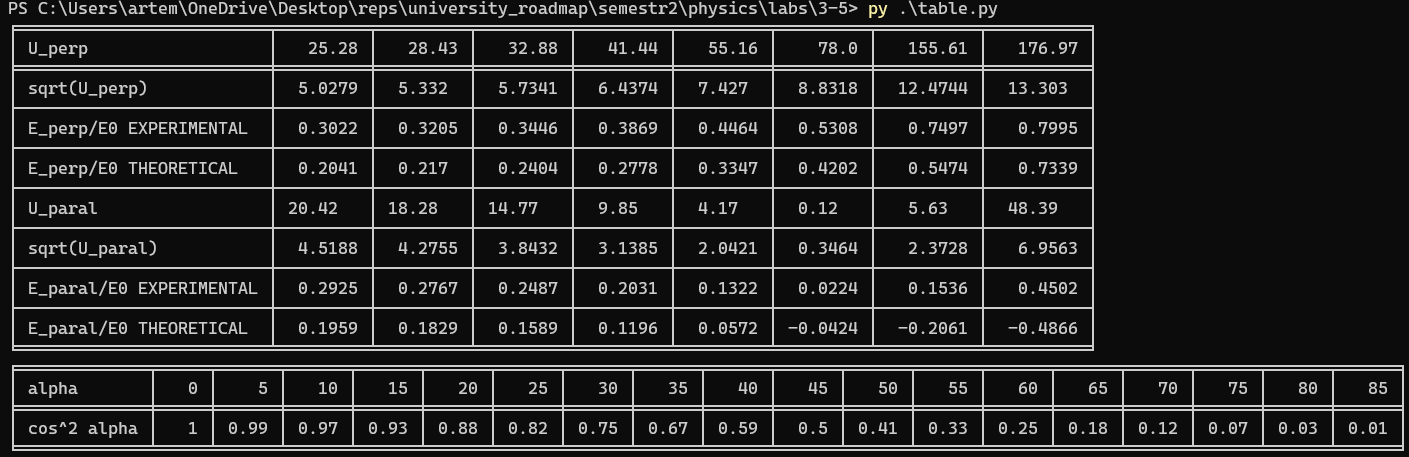
\includegraphics[width=1.0\textwidth]{result.png}
    \end{figure}

\end{document}